\documentclass[11pt,final]{article}%

% Page
\usepackage[margin=2.54cm, letterpaper]{geometry}
\usepackage{rotating}
\usepackage{epstopdf}
\usepackage{pdflscape}
\usepackage[english]{babel}
\usepackage[strict]{changepage}

% Math
\usepackage{amsthm,verbatim, amsmath, amsfonts, amssymb, mathtools, cases}
% \usepackage[toc, page, title, titletoc]{appendix}
\usepackage{type1cm}
\usepackage{bm}
\usepackage{courier}
\usepackage{relsize}
\usepackage{float}
% \usepackage{flafter}
\usepackage{graphicx}
% \usepackage[percent]{overpic}

% Tables & floats
\usepackage{tabularx, siunitx, tabu, array, longtable, multicol, booktabs,
	multirow, threeparttable}
\usepackage{siunitx}
\usepackage{ragged2e}
\usepackage[labelfont=bf,skip=0pt]{caption,subfig}
\usepackage[doublespacing]{setspace}
\usepackage{fancyhdr}
\usepackage{pageslts}
%\usepackage{endfloat}

% Quotes
\usepackage{dirtytalk}
% \usepackage{csquotes}

% Bibliography management
\usepackage{natbib}
\usepackage{har2nat}
\usepackage{breakcites}
\usepackage{xr-hyper}
\usepackage{hyperref}

% Cross-referencing
\usepackage{zref-xr,zref-user}
\zxrsetup{toltxlabel}
\zexternaldocument*{sup-material}

%\usepackage{nameref}
\usepackage[textsize=scriptsize,colorinlistoftodos, color=yellow]{todonotes}
% Allows using endfloat with sidewaystable (see endfloat doc)
% \DeclareDelayedFloatFlavor{sidewaysfigure}{figure}
% \DeclareDelayedFloatFlavor{sidewaystable}{table}

\setcounter{MaxMatrixCols}{30}
\providecommand{\U}[1]{\protect\rule{.1in}{.1in}}
\newcolumntype{C}{>{\centering\arraybackslash}X}
\newcolumntype{L}{>{\raggedright\arraybackslash}X}
\newcommand\mC[2]{\multicolumn{#1}{C}{#2}}
\newcommand{\vect}[1]{\bm{#1}}
\geometry{verbose,headsep=0in}

\title{The role of capital in the diffusion of bank failure}
\author{ecarlevaro }
\date{December 2020}


\begin{document}

\maketitle

\section{Abstract}
Banking crises are contagious: healthy banks can be negatively affected by the behavious of unhealthy banks. Banking crises spread among firms similar to a infectious disease. We model banking crises using a standard susceptible-infceted-recover (SIR) model and then we link the structural parameter from this model to the distribution of bank capital in each crisis. Results suggest that an increase in the size-wighted average of capital ratio of XX reduces the number of banking failures by YY. A change in the capital ratio in a big bank is not the 

\section{Introduction}
How does a shock transmitt through the economy? Understanding the propagation of a shock reveals whether the underlying structure of the economy amplify or reduce the initial shock. We consider the propagation of bank failures through the Argentinian financial system.
Bank failures are socially expensive and can lead to a meltdown of the financial system and the macroeconomy. 
In the presence of financial frictions, the financial structure of individual banks determines its failure probability. For instance, capital in the form of equity is state-invariant contract: shareholders cannot withdraw their capital when bad outcomes are realised, in contrast, a deposit contract enables depositors to run in the bad state. 

There is a big and old literature that analyzes whether banks with higher capital are less likely to fail. \say{Most of the literature on bank failure concentrates on accounting variables. Virtually all such studies find that low capital ratios raise the
probability of bank failure. }, \say{(e.g., Lane, Looney, and Wansley, 1986; Cole and Gunther, 1995, 1998; Wheelock
and Wilson, 1995, 2000; Calomiris and Mason, 1997, 2003; Elsinger, Lehar, and Summer, 2006; Schaeck, 2008, Cole and White, 2012; Knaup and Wagner, 2012; Admati, DeMarzo, Hellwig, and Pfleiderer, 2013; Berger and Bouwman, 2013; DeYoung and Torna, 2013; Berger, Imbierowicz, and Rauch, 2016)} Almost all the literature confirm that higher bank capital reduces the probability of failure. This means that \textit{on average} bank capital has positive marginal returns. As explained above, unregulated banks are on average undercapitalised.

Individual banks may choose a suboptimal equity level because each bank does not face the total cost of its failure. This ocurrs when contagion is possible: a bank failure affects other banks failure rates.  As a result, capital regulation has emerged to 

Concodrdingly with the presence of contagion, bank failures rarely occurr isolated but rather are clustered in time as shown below

\begin{table}[]
    \centering
    \begin{tabular}{c}
         \textbf{USA}. Quarterly bank exits as a percentage of total banks in the quarter \\
         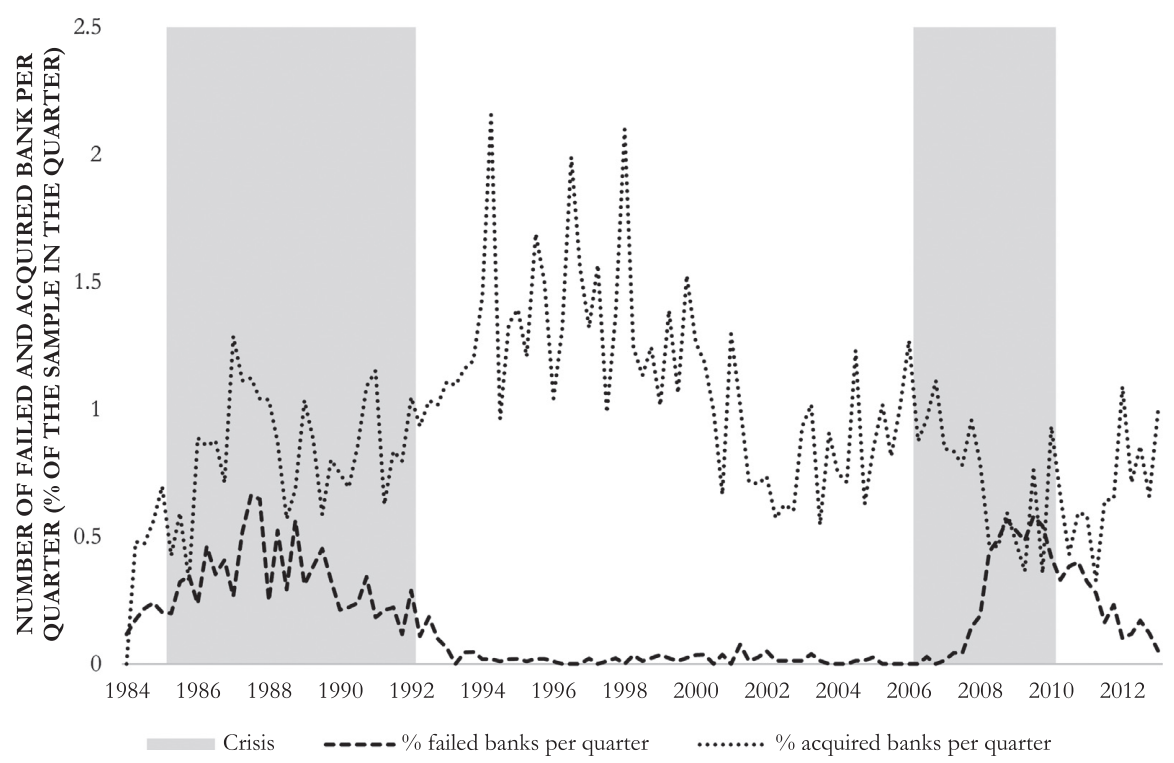
\includegraphics[width=\textwidth]{graphs/USA_Spokeviciute Keasey V Bank exits.png} \\
         Source: \cite{SpokeviciuteKeaseyVallascas2019} \\
        \addlinespace
          \textbf{Spain}. Banking crises in grey \\
         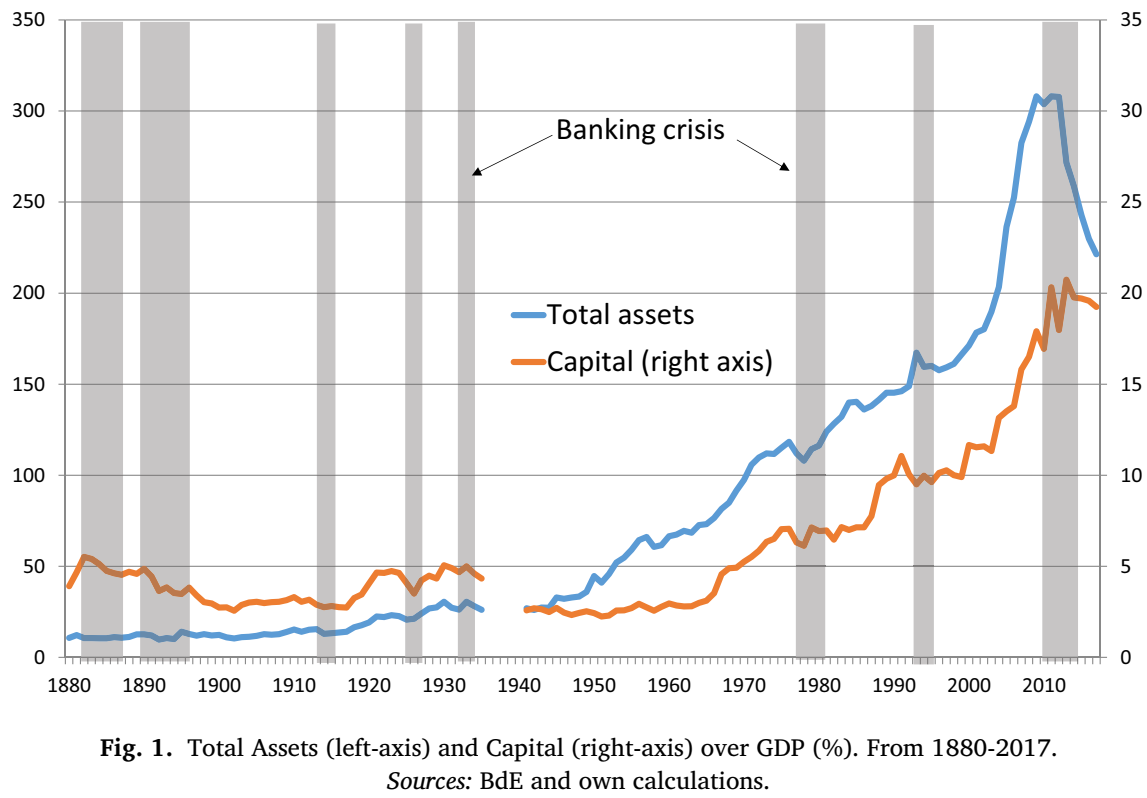
\includegraphics[width=\textwidth]{graphs/Spain banking crises.png}
          Source: \cite{BedayoEstradaSaurina2020} \\
    \end{tabular}
    \caption{Caption}
    \label{tab:my_label}
\end{table}
This suggests some propagation or contagion among banks.

Contagion is a distinctive feature of banks from other firms in the economy. If Coles has problems, Woolworths increases its revenuyes, this does not occur in the banking sector.  There are at least 4 channels that spur contagion of bank failures: bank runs, fire sales, interbank markets and correlated risks. Bank runs stem from the inability of bank creditors to distinguins a illiquid bank from an unsolvent one. In such scenario, failure of an insolvent bank might trigger a run on the liabilities of a solver but illiquid bank \cite{DiamondDybvig1983}. Fire-sales is another mechanism for contagion: the liquidation of assets from bank F assets reduce asset prices in the market thus reducing the value of these assets in bank H balance sheet  \cite{Walther2016}.
A third channel is the inter-bank market: if an 'important' bank resides from this market it can impared the funciton of the market (in the extremthe market could freeze as during the GFC). A dry interbank market reduces abilities for all banks to withstand an idiosycratic shock, since this shock cannot be easily transfer to other banks. 
A fourth mehcanism arises when banks invest in similar projects and thus their loans portfolios are highly correlated \cite{FarhiTirole2012}.





The above empirical literature does not consider the role of contagion in the estimation of capital and failure.

We disentangle the effect of bank capital on its own failure probability from the contagion or spillover effect from other banks capital on its own failure probability. We first estimate the linkages among banks using balance sheet data. We then use a duration model expanded with the linkages and the observed bank failures. This allos disentangling the effect of a change in capitalisation of a bank on its ouw failure probability and the spillover effect from other banks to whom it is linked. 

Our results  concerns investors, rgulatores and central banks concerned about financial stability. 
 A regulatro is concerned on whether banks will freely choose the optimal contract for the financing. FOr instance, the established European Single Resolution Board regulation in the European Union  aims at making systemic banks 'resolvable'. This mean that even if a big bank fails, it is possible to continue its operation without resorting to taxpayers money. The most common of way of resolution is a bank acquisition. This, however, requires that there is a acquire bank which is not already affected by the failure. Bank resolvability thus require knowledge of the linkages among banks and the role of these linkaes during a crisis. 
 \todo[inline]{\cite{Labbe2017} Banco Popular restructuring proves SRB can work}
 

++++++++++++++

Given bank capital choices capital regulation forces each bank to hold a minimum lelve of equity. This enforces a minmum bound on the \textit{individual} failure probability of a bank, whihc is called microprudential regulation.

To reduce contagion effects Micro- and macro-prudential regulation use common tools (capital requirements, cash reserve or liquid asset requirements, risk weighting of assets, provisioning rules, etc.) but have different goals. Micro-prudential regulation focuses on the safety and soundness of individual banks. Macro-prudential regulation focuses on stabilizing the banking system as a whole, for example, by seeking to limit systemic contagion by requiring money center banks to maintain higher cash reserves than peripheral banks, by requiring larger banks to maintain higher capital ratios, or by leaning against episodes of very rapid lending growth by increasing minimum capital ratio requirements. (CALOMIRIS, CARLSON, 2015)


What is the probability that a bank fails?

 
 
 specific contracts prevent bank failures. 
Bank crises are contagious



\section{Stylized facts}

\subsubsection{Individual capital ratios are relevant in a network}
In the presence of contagni, what determines the spread and size of crisis are not the individual capital ratios but its weighted  distribution in which the weights depend upon the importance (centrality) of each bank in the system. The GFC  \say{underlined the need to move from a pure microprudential view of capital requirements (i.e., focused only on the capital level at each individual bank) to a more comprehensive or holistic view of capital (...) That is, policy makers must pay attention to the aggregate bank capital ratios and to how they evolve along the business cycle.}

\subsection{Contagion as an externality}
\todo[inline]{In the fire-sales literature the word is externality but it could also be spilover effect.}
A highly interconnected banking system allows banks to share capital. However when a bank fails, since the cost is shared by all banks due to contagion, some banks may optmially hold lower level of capital than optimal. This negative externality conversely works in the opposite direction. A bank can shield from contagio by choosing an appropiate strucutre of ocntactracts. For example, a bank could choose a high cpaitalziation ration than its competitiors to reduce its probability of failure. Since this reduction also marginally reduces the probaiblity of failure of other banks through contagio, thei higer capitalizaion of a bank creates a positive externalitiy for other banks. This suggest that in equilibrium each bank will choose a level of capitaliation  lower than the socially optimal.

A well-capitalised bank may fail if its neighbors are poorly-capitalised. 

The above facto implies that a regression of the proportion of failing banks on its capital level will suffer from a ommited variable problem.

We need to identify for each bank $i$:
\begin{enumerate}
\item Its neighbors.
\item The capital level of these neighbors. 
\end{enumerate}

A weighted-average of bank capital ratios. 
\say{It turns out that the minimization of (standard measures of) individual risk can often increase the level of systemic risk, which in turn can hurt individual financial entities1,2} \cite{SquartiniVanGarlaschelli2013}

\subsection{Marginal effects: direct and indirect}
The object of interest is the effect of a indvidiaul bank variable on its own surviaval probaiblity {keeping constant} the contagion or network effect. Denoting the $(N \times 1)$ vector of individual banks probabilities at time $t$ by $\vect{y}_{t} := [ y_{i,t} \, \cdots y_{N, t}]$ and let $X_{t}$ be the $(N \times K)$ matrix of each bank variable such that  column $i$, $X_{,i}:= [x_{i,1} \cdots x_{i, k}]_{t}$ . This matrix contains, for example, the capital ratio of each bank at time $t$. 

A standard approach in the literature is formulate a model such that:
\begin{equation}
\vect{y}_{T} = f( X_{t} \vect{\beta}) + \vect{\epsilon}
\label{basic_model}
\end{equation}
where the failure probabilit is only computed at time $T$, the $f(\cdot)$   function can be a linear function or exponential, $X_{t}$ is usually lag in time with respect to $T$ and the $(N \times 1)$ vector $\epsilon $ is uncorrelated among banks. 

Acknowleding the contagions among banks implies that the assumption of independent errors $\epsilon_{i, t}$ is not suitable. Recongnising the contagion implies drawing a specific dependance among banks.

At the same time, the model in equation (\ref{basic_model}) does not consider \textit{when} a bank fail. It is reasonable to expect that if a well-connected bank (a 'central' bank) fails at the beginnig of the time the dynamic of bank failure will be different that if small banks start failing. 

Recognising the dependance and the time of failure as properties of bank failures  implies that each bank failure probabiliy depends upon it own variable as well as other banks.

Let a matrix $W$ define the relationship among banks.

Then a more suitable model will be: 

\begin{equation}
\vect{y}_{t} = f(X, W) \, + \, W \vect{\epsilon}_{t}
\end{equation}

Let the average probabiliy of failure at time $t$  be $\mathbb{E}[y_{i}]_{t} $ where the expectation is taken over banks, , the interest lies in the partial derivative $\frac{\partial \mathbb{E} [{\vect{y}}] }{ \partial x_{i, k}} $. To identify this partial derivative the model requires to keep constant the contagion or indirect effect, that is $\frac{\partial \mathbb{E} [{\vect{y}}] }{ \partial x_{j, k}} $ where $j \neq i$ .
In the model above there are two effects: a direct effect of each bank covariate on its survival rate and an indirect or contagion effect that come through the network. Specifically, the survival probability of bank $i$ depends upon its own capital structur, as well as the capital structure of its 'neighbours' banks. 
From this follows that for each bank $i$ the marginal effect is different depending on who its neighbours are (tecnically, the 'centrality' of them in the graph). 

Hence the effect of each own variables on the probability of failures are:
\begin{equation}
\left( \frac{\partial \mathbb{E}[\vect{y_t}]  }{\partial x_{1k}} \, \cdots \, \frac{\partial \mathbb{E}[\vect{y_t}]  }{\partial x_{Nk}} \right) = 
\begin{bmatrix}
\frac{\partial \mathbb{E}[\vect{y_{1,t}}]  }{\partial x_{1k}}	&	\cdots 	&	\frac{\partial \mathbb{E}[\vect{y_{1,t}}]  }{\partial x_{Nk}}	\\
\vdots 	&	\ddots 	& \vdots  \\
\frac{\partial \mathbb{E}[\vect{y_{N,t}}]  }{\partial x_{1k}}	&	\cdots 	&	\frac{\partial \mathbb{E}[\vect{y_{N,t}}]  }{\partial x_{Nk}}	\\
\end{bmatrix}
\label{eq:marginal_effects}.
\end{equation}
The vector on the left contains the effect that a marginal change in the $k$-variable of each and \textit{every} bank contributes to the mean survival probability. The fact that every bank contributes to this probability is the sense that we identify the contribution of each bank to the \textit{systemic risk}. Notice that these derivatives are not equal in magnitude but instead their size depend upon the  weighting matrix $W$ (that is, the relative position of each bank in the graph).

The matrix on the right contains in its first row the effect on bank $1$ of a change in its own level of the $k$-variable and a change of the others bank level of the $k$-variable on its own survival rate.  Each column of the matrix instead contans the effect of each $k$-variable on \textit{all} banks expected survival rate.

Recognising the role of the dependence and time of failure in order to estimate the marginal effects in equation (\ref{eq:marginal_effects}) we propose to use the model from \cite{ElhorstHeijnenETAL2017}.

\section{Methodology}

\subsection{MOdel specification}
The goal of the econometric model is to capture both aforementioned effects on a bank failure probability: the direct effect due to its own capital structure and the contagion effect. 

At each time $t$, bank $i$ can be in two states:
\begin{equation}
y_{i, t} =
\begin{cases}
	0 &	\text{Active at time }t, \\
    1 &	\text{Failed (bankruptcy or liquidation) at time }t, \\
\end{cases}
\end{equation}
Banks that fail at time $t$ are removed from the sample.  Denoted by $N^{0}_{t}$ active banks at time $t$ and $N^{1}_{t}$ failed banks by time $t$, the total number of banks is $N = N^{0}_{t} + N^{1}_{t}$.


A bank failure probability $y^{*}_{i,t}$ is not obvservablle but we observe failures at time $t$,  $y_{i,t}$. Define the unnobservable $N_{t}^{0} \times 1$ vector $\vect{y^{0*}_{t}}$ which contains the probability of failure of active banks at time $t$ and the $(N_{t}^{1} \times 1)$ vector $\vect{y_{t}^{1}}$ which fails at time $t$. The effect of bank failures in the second vector are intermediate by the 'distance' of the failing banks to the active banks.

The association among banks at time $t$  is captured by the spatial weight (or adjacency) matrix $W_{t}$:
\begin{equation}
W_{t} = 
\begin{bmatrix}
	0			&	w_{1, 2}	&	w_{1,3}		&	\cdots	&	w_{1, N}	\\
    w_{2,1}	&	0				&	w_{2,3}				&	\cdots	&	w_{2, N}	\\
    w_{3,1}	&	w_{3, 2}	&	0				&	\cdots	&	w_{3, N}	\\
    \vdots 	& \vdots		&	\vdots		&	\ddots	&	\vdots	\\
    w_{N,1}	&	w_{N, 2}	&	w_{N,3}		&	\dots	&	0	\\
\end{bmatrix},
\end{equation}

where the time subscript were omitted in the components of the matrix. 

We want to capture the different effect that a failed bank has on the surviving banks. Thus in the model this matrix is divided into two submatrices: $W^{00}_{t}$for the relationships between active banks, and $W^{01}_{t}$ for the relationships between active banks and failed banks at time $t$. This division enable capturing the diffusion  effect of a failure: a fail banks affects its closest neighbours and this in turn reverberate in the system of active banks. 

Notice the dimesion of the adjacency matrix evolves over time. For each $t$, $W^{00}_{t}$ is $(N^{0}_{t} \times N^{0}_{t})$ and $W^{01}_{t}$ is $(N^{0}_{t} \times N^{1}_{t})$.

The capital ratio for each bank and all other indibidual covariates are stored by the $(N \times K)$ matrix $X$.

At each $t$ the failure probability of all active banks is updated based on the failures of that time and the covariates in $X$. 

The regression equation is:
\begin{equation}
	\underbrace{\vect{y}^{0*}}_{N \times 1} = \alpha \vect{1} \,+\, \rho_{1}  W^{00}_{t} \vect{y}^{0*}_{t} \,+\, \rho_{2} W^{01}_{t} \vect{y^{1}_{t}}  \,+\, X_{t} \vect{\beta} \,+\, \vect{\epsilon^{0}}_{t}
    \label{eq:stc_form}
\end{equation}
where $\vect{1}$ is a vector of 1s, the $\vect{\epsilon}$ is a $N \times 1$ vector of idionsyncratic errors such that $\mathbb{E}(\vect{\epsilon} | \vect{x}, W)=0$. 
The parameters are the $N \times 1$ vectors $\alpha, \rho_1, \rho_2, \beta$ . 

The vector $\rho_1$ captures the interaction effect among active banks.  This interaction effect is an endogenous variable in equation (\ref{eq:stc_form}) since the variable $y_{t}^{0*}$ is unobservable. The parameter $\rho_2$ instead captures the interaciont of fail banks with active banks. $\beta$ captures the contribution of each bank own covariates to the failure probabilities of all banks. 

Given enough macro controls (and fixed-effects?) we can mitigate any cross-correlation among panels such that $\mathbb{E}(\epsilon_{i} \epsilon_{j}) = 0$. 

\subsection{Marginal effects}
The coefficients from the above model cannot be interpreted as the marginall effects due to the nonlinearity of hte function . 

\cite{Elhorst2017} condier the marginal effect from the above model as:
\begin{equation}
\left( \frac{\partial \mathbb{E}[\vect{y_t}]  }{\partial x_{1k}} \, \cdots \, \frac{\partial \mathbb{E}[\vect{y_t}]  }{\partial x_{Nk}} \right) = 
\begin{bmatrix}
\frac{\partial \mathbb{E}[\vect{y_{1,t}}]  }{\partial x_{1k}}	&	\cdots 	&	\frac{\partial \mathbb{E}[\vect{y_{1,t}}]  }{\partial x_{Nk}}	\\
\vdots 	&	\ddots 	& \vdots  \\
\frac{\partial \mathbb{E}[\vect{y_{N,t}}]  }{\partial x_{1k}}	&	\cdots 	&	\frac{\partial \mathbb{E}[\vect{y_{N,t}}]  }{\partial x_{Nk}}	\\
\end{bmatrix}
=
diag[ \phi(\hat{\vect{y}}^{0}_{t}) ] \, (I - \rho_{1} W_{t}^{00})^{-1} \, I_{N} \beta_{k}
\label{eq:marginal_effects}
\end{equation}
where $\eta = (I - \rho_{1} W_{t}^{00})^{-1} \, (\rho_{2} W_{t}^{01} \vect{y_{t}^{1}} \,+\, X_{t}^{0} \vect{\beta} )$ are the predicted values for $\vect{y}^{0}_{t}$.

From the 


Thus the failure probability is regarded as a latenet variable.
Let the  $\vect{y}$ be a  which contains the exit situation of each bank. 
For each $t$, the $N^{0}_{t} \times 1$ vector $\vect{y^{0}_{t}} = [y^{0}_{i, t} \, y^{0}_{j, t} \, \cdots \,  y^{0}_{N_{t}^{0}, t} ]$ collects all active banks. 


Solving for $\vect{y}$,
\begin{equation}
\vect{y} = \alpha (\vect{I} - \beta \, W \, )^{-1} \,+\, (\vect{I} - \beta \, W\, )^{-1} (\eta \vect{I} + \gamma W) \, \vect{x}\,  + (\vect{I} - \beta \, W\, )^{-1} \vect{\epsilon}
\end{equation}
where $\vect{I}$ is the identifity matrix of order N.

\todo[inline]{This is Girish's point. What you 'identify' as network effects is just the macro shock propagating through banks.}

\subsubsection{Stability of W}
We assume a constant relation among banks. Two reasons motivate this. First, much of the interdependence among banks is builts on reoaltionshiop lending. Most of the deals among banks are over-the-counter trades that hinge upon mutual knowledge. Relationship lending takes time to build so it will not be quickly created. Bu9ilding new relationhip may presumably be less likely during crisisi time when asummetric of information between banks are amplified.  
Second, evidence using overnight interbank loans by \cite{Forte2020} suggest that the network evolves smoothly. In the case of the 2008 crisis, he observes changes towards a reduction in the nodes and edges.  This implies that less banks were able to trade during the crisis (W became more sparse) reducing the possiblity for a bank to hedge any shock in others. 
We, in contrast, assume a fixed W at the beginning of each crises. Because of this, we interpete our estimated effects as a lower bound. If during the crisis the network shkirns, distrssed banks are less able to find financing and healthy banks are less able to be affected. 

Notice that W is indeed changing over time as we remove failing banks, that is the network is updated every time a bank fails. 





The above discussion

\subsection{Financial creses precede recession}
Financial crises usually trigger recession rather than the other way around. Bank capitalisation (leverage) and loans growth is usually referred as  a cause of business cycles. That is, bank decisions can create recessions.

\subsection{Goverment subsisdy}
While banking is a heavily regulated sector it is also subsidised. Either through a deposit insurance scheme or government-sponsored bail-out.

\subsection{Banking crises are endemic}.
Banking crises are not extraordinary '4-sigmas' events: while these do not occurr frequently, they ocrurr systematically across both develop and emerging markets.

\subsection{Failure is predictable}
There is abundant literature that finds accounting measures as strong predictor of failures. Starting with Altman in 1968 for non-financial firms to \citeasnoun{BergerBouwman2013}, \citeasnoun{SpokeviciuteKeaseyVallascas2019}

\subsubsection{A failed bank is not affected by alive banks}
Once a bank failed, it is not affected by the outcome of healthy banks. Thus it makes sense to remove it from the sample.


\subsection{Probability of failure}
The integral under the epidemic curve $\int_{0}^{\infty} i(t) dt $ is similar to ae scalar version of the probability of failure in the classic probit model. 
Capital regulation by redicng the infection rate can actually 

The traditional problit/logic metohodology treats its outbreak as independent ignoring the regularity of banking crisises and that the unbalanced on the panel is not random but instead the banks in the last crises (outbreaks) surveved the previous. 

\subsubsection{Heterogeneity}
The heterogeneity can be introduced in two ways. Through 'age-groupps' and 'contact frequency'. Age groups for bank we can consider as capital levels: banks with higher capital level are less susceptible for becoming infected and failing. Contact frequency as the size of the bank: bigger banks have more chances of transmitting the diseases for two reasons: first htey may have more finaical relationsihps with other banks (for instance lending to smaller banks in the interbank market). Secondly, if a big bank fails it isi more likely that stakeholders of smaller banks panic and run on their assets. 

Ignore the systemic risk
given the contagion, the probability of failure for a bank depend upon the other banks . SIR models endoneously capture this dependance by considering the number of infeceted indivuials at each point in time: the probability of failue (infection) evolves with the number of failing institutions. This capture the systemic componenet as well as the idiosyncractic component of the risks in a banking crisis. 

.
 The optimal level of capital $k_{i, t}$ for a bank to withstand, say, 95\% fo the shocks (a Valure-at-Risk) depend on the capitalisationm of the other $k_{j,} \neq i$ banks. In other words, assum,e that the same level of capital will provide the same protecion across countries regardless of the capitalisaton of the other banks. 



Many of the above stylized facts for banks failures are the same as disease transmission in a population: positie and negatie feedbanks about individuals, time delays in the buildup on risks (infected people or risky assets), nonlinearities, stochastic events and individual heterogeneity.

A bank crises shares manny commonatility with a endemic infectious disease: its spreads rapdilty increasing and then decreasing, outbreaks occurrs with certain reuglarity, some individuals die as a result, some idnividuals are more susceptivel than others, there are feedback effects (extenratilites) for individual actions, exogenius interventions can change the outcomes (ie, social distacning measures, rgulation or banks bail-in), changes in population seed the seed for the new outbreak. 
\subsection{Differential equation models}

Each individual is classified into a compartiment: susceptiel

bank's creditors Banks are different to oteheA distinctive feature of ban

There is a theory which states that if ever anyone discovers exactly what the Universe is for and why it is here, it will instantly disappear and be replaced by something even more bizarre and inexplicable.
There is another theory which states that this has already happened.

\section{Literature review}

Debate on the uniquness of the GFC
There is a debate on whether the predictability of banks failures during the GFC is lower than in previous crisis. The metodology used, however, relies on logit or probit models without accounting for systemic risk and contagion. 
During the GFC contagions was at the heart of the crisis after the interbank, certificate of depotis (CDS) and mortage-backed securities frozen \cite{GortonMetrick2012}.
\subsection{Probit is Popular}
All the literatre uses variane of a probit model.

\section{Network}
\subsection{Stability}


\begin{figure}[h!]
\centering

\includegraphics[scale=1.7]{universe}
\caption{The Universe}
\label{fig:universe}
\end{figure}

\section{Conclusion}
``I always thought something was fundamentally wrong with the universe'' \citep{adams1995hitchhiker}

\bibliographystyle{plain}
\bibliography{references}
\end{document}
